\chapter{Results}
\section{\label{section:Parameter setup for Change Point Detection Methods}Parameter setup for Change Point Detection Methods}
As we know that our change point detection algorithms depends on the values of 3 different parameters- sliding window size, sliding amount and number of change points, we have systematically varied these parameters to obtain the optimum efficiency of change point detection methods for all three species. 
To tune the sliding window size for each species, we have varied it from 40-120 seconds with an interval of 10 seconds. We have varied the sliding amount from 10-30 seconds with an interval of 10 seconds. For each of the species we have observed the simulations visually to track down, how many times ants discover a particular type of pile and noted that number. We put that data on the algorithm as a statistical parameter.\par 
After comparing the efficiency of all this settings we have tuned this parameters for each of the species. Table $4.1$ describes the parameter settings of simulations for each of the species
\begin{table}[h]
	\begin{center}	
\begin{tabular}{|p{0.2\textwidth}|p{0.11\textwidth}|p{0.12\textwidth}|p{0.12\textwidth}|p{0.25\textwidth}|}
	\hline
	\textbf{Species} & \centering \textbf{Pile} & \centering \textbf{Window Size} & \centering \textbf{Sliding Amount} & \centering \textbf{Mean Number of Change Points} \tabularnewline
	\hline
	\multirow{3}{0.2\textwidth}{\textit{P. Desertorum}} & \centering 1 & \centering 80 & \centering 20 & \centering 6 \tabularnewline 
	\cline{2-5}|
	& \centering 4 & \centering 80 & \centering 20 & \centering 4 \tabularnewline
	\cline{2-5}
	& \centering 16 & \centering 80 & \centering 20 & \centering 2 \tabularnewline
	\hline
	\multirow{3}{0.2\textwidth}{\textit{P. Maricopa}} & \centering 1 & \centering 70 & \centering 20 & \centering 2 \tabularnewline 
	\cline{2-5}
	& \centering 4 & \centering 70 & \centering 20 & \centering 5 \tabularnewline
	\cline{2-5}
	& \centering 16 & \centering 70 & \centering 20 & \centering 4\tabularnewline 
	\hline
	\multirow{3}{0.2\textwidth}{\textit{P. Rugosus}} & \centering 1 & \centering 60 & \centering 10 & \centering 4\tabularnewline 
	\cline{2-5}
	& \centering 4 & \centering 60 & \centering 10 & \centering 4 \tabularnewline
	\cline{2-5}
	& \centering 16 & \centering 60 & \centering 10 & \centering 4 \tabularnewline
	\hline
\end{tabular}
\end{center}
	\caption{Environmental Setup of simulation for three species}
\end{table}
\section{\label{section:Results from Simulation}Results from Simulation}
%\subsection{\label{Pheromone Only Parameters}Pheromone Only Parameters}
We configured the simulation settings as close as we can with the experimental setup of \textit{P. Rugosus}, \textit{P. Maricopa} and \textit{P. Desertorum}. Then we have compared the result of method \textit{alpha}, \textit{beta}, \textit{gamma} and \textit{delta}. based on the time between a pheromone laying event followed by the detection of change point.\par 
Figure $4.1$ compares the results of four different methods on a pheromone only simulated environment for \textit{P. Rugosus}. We can see that, \textit{Method $\alpha$} detects change points which is closer to the pheromone laying event. The result of \textit{Method $\beta$} is closer to the \textit{Method $\alpha$}, but {Method $\gamma$} and {Method $\delta$} doesn't perform well in this environmental settings.\par 
\begin{figure}[H]
	\includegraphics[width=\textwidth,height=0.5\textheight]{PheromoneOnly/AllPlot.png}
	\caption{Comparison of change point detection method for pheromone only parameters. Outliers are skipped to provide a better perception of differences. The time in seconds represents the difference between a pheromone laying event followed by a detection of change point in the foraging rate.}
\end{figure}
We have illustrated the result of \textit{constant detrending} method in figure $4.2$. The average difference of pheromone laying event followed by a change point detection for \textit{constant detrending} method is $47.5$, $60$ and $81.5$ for one pile, four large piles and sixteen piles. It is also observed that, the range of time difference between a pheromone laying event followed by a change point detection event is also significantly reduced.\par 
We observe similar phenomenon for \textit{P. Maricopa} and \textit{P. Desertorum}. The box plots of comparison for these two species are provided in the Appendices. The outliers are removed from the figure to make the figure more visible. The detailed figure with the outliers are provided in the appendices.\par 

\begin{figure}[H]
	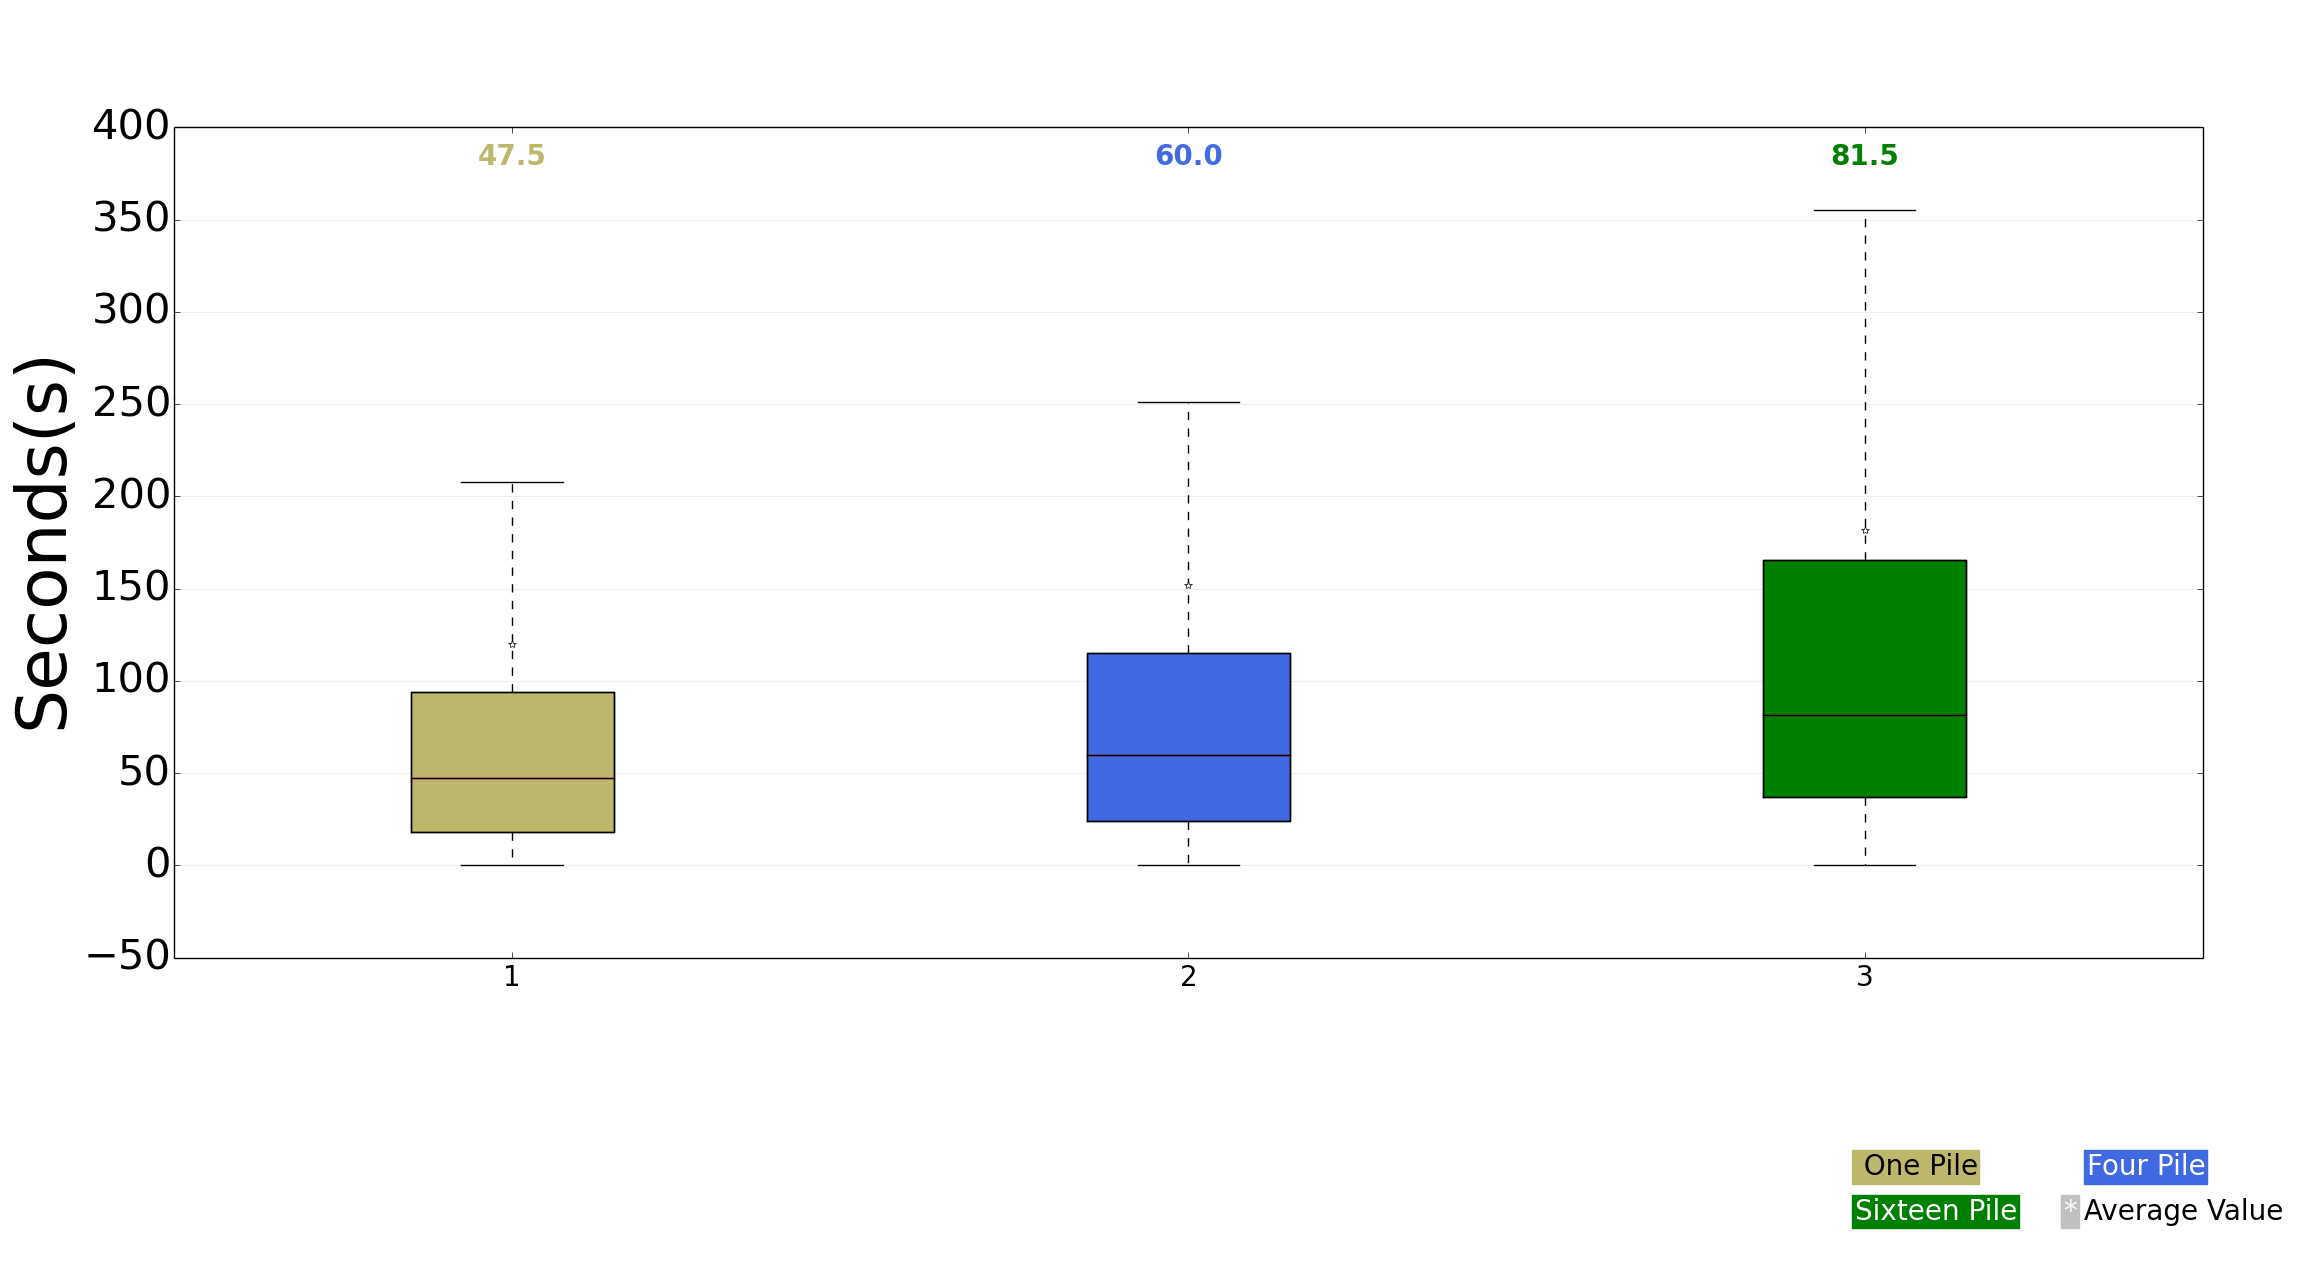
\includegraphics[width=\textwidth,height=0.5\textheight]{PheromoneOnly/ConstantWithNoOutlier.png}
	\caption{Enlarged view of efficiency of \textit{constant detrending} method. The time in seconds represents the difference between a pheromone laying event followed by a detection of change point in the foraging rate.}
\end{figure}


We have also evaluated four different methods based on the four categories mentioned in section $3.7$.
As we can see from figure $4.3$ in \textit{constant detrending} method, $15\%$ of the time change points are detected within 10 seconds of laying pheromone, whereas, in \textit{linear detrending} method, it is only $9\%$. \textit{Constant detrending} method also has significant improvement over \textit{linear detrending} method in \textit{Catagory B}. $74\%$ of the time, changes points are detected with eleven to three hundred seconds of laying pheromone while using \textit{constant detrending} method, on the other hand, using \textit{linear detrending} method it is only $50\%$. In \textit{catagory C} the error is $6\%$ for \textit{constant detrending} method, whereas, it is $21\%$ for \textit{linear detrending} method. \par
\begin{figure}[h]
	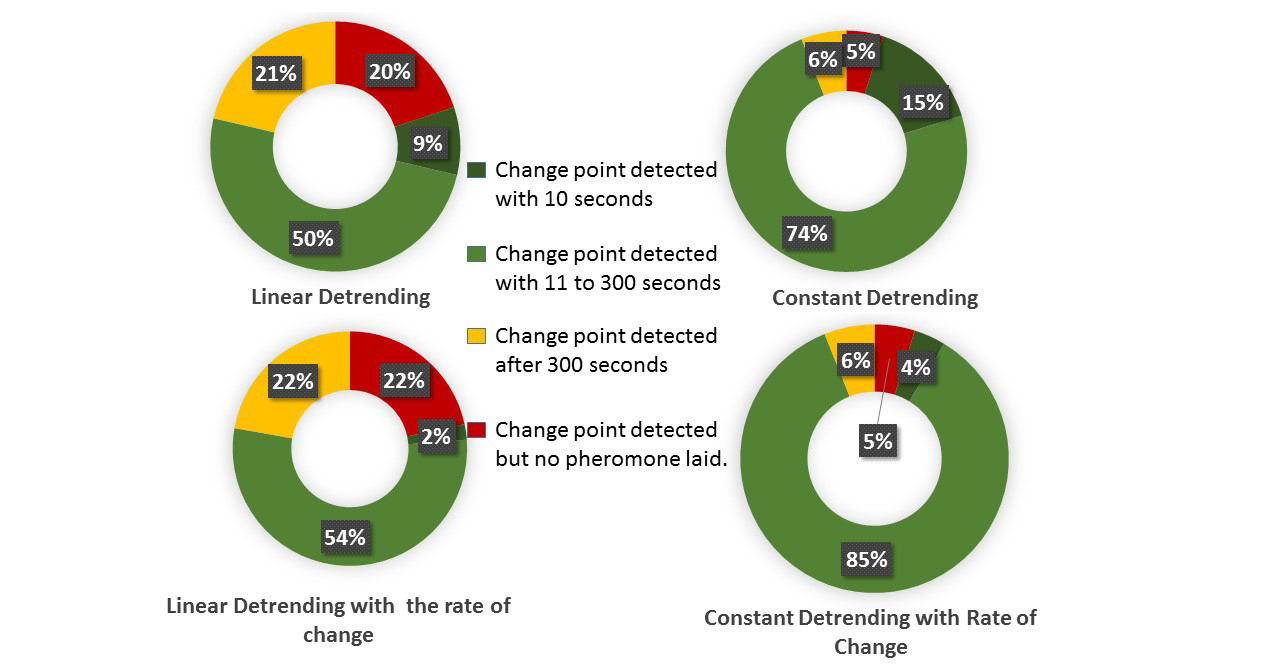
\includegraphics[height=0.35\textheight]{DonutCharts/Slide2.JPG}
	\caption{Efficiency chart for Change Point Detection Methods on a large pile of 256 seeds. This result is generated from the simulated data of pheromone only environment, configured for \textit{P. Rugosus}}
\end{figure}
Performance of \textit{constant detrending method} and \textit{constant detrending method with difference in rate} is similar. if we consider categories A and B. But \textit{Method $\alpha$} does significantly better than \textit{Method $\beta$} in detecting change points for four piles and sixteen piles in the simulated environment.\par
From figure $4.4$ and figure $4.5$ we can observe that, the performance of \textit{Method $\alpha$} combined in category A and B is better than performance of \textit{Method $\beta$} combined in these two categories. Also from figure $4.4$ and $4.5$ we can see that \textit{Method $\alpha$} does better in category C than \textit{Method $\beta$}. \par
If we look at the performance of the four methods over these categories in phermone only simulated environments, for \textit{P. Maricopa} and \textit{P. Desertorum} we observe similar pattern of performances. The results for \textit{P. Maricopa} and \textit{P. Desertorum} provided in the appendices.\par   

\begin{figure}[h]
	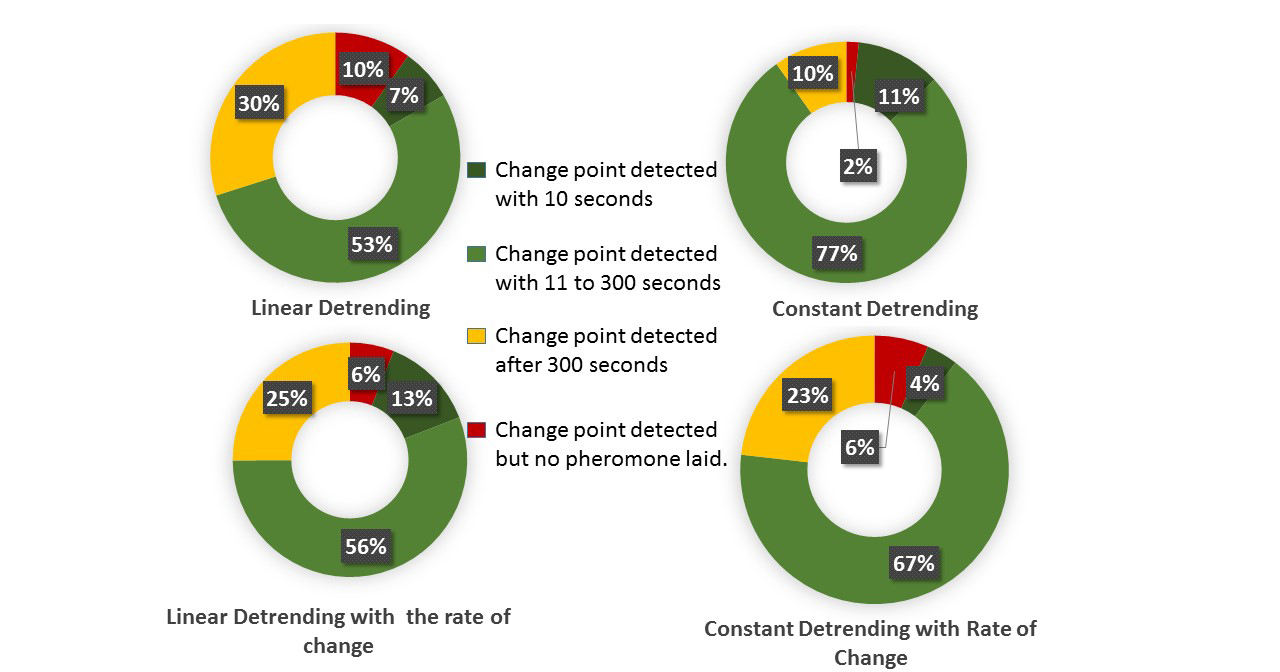
\includegraphics[width=\linewidth, height=0.4\textheight]{DonutCharts/Slide3.JPG}
	\caption{Efficiency chart for Change Point Detection Methods on four medium  piles of 64 seeds. This result is generated from the simulated data of pheromone only environment, configured for \textit{P. Rugosus}}
\end{figure}
\begin{figure}[H]
	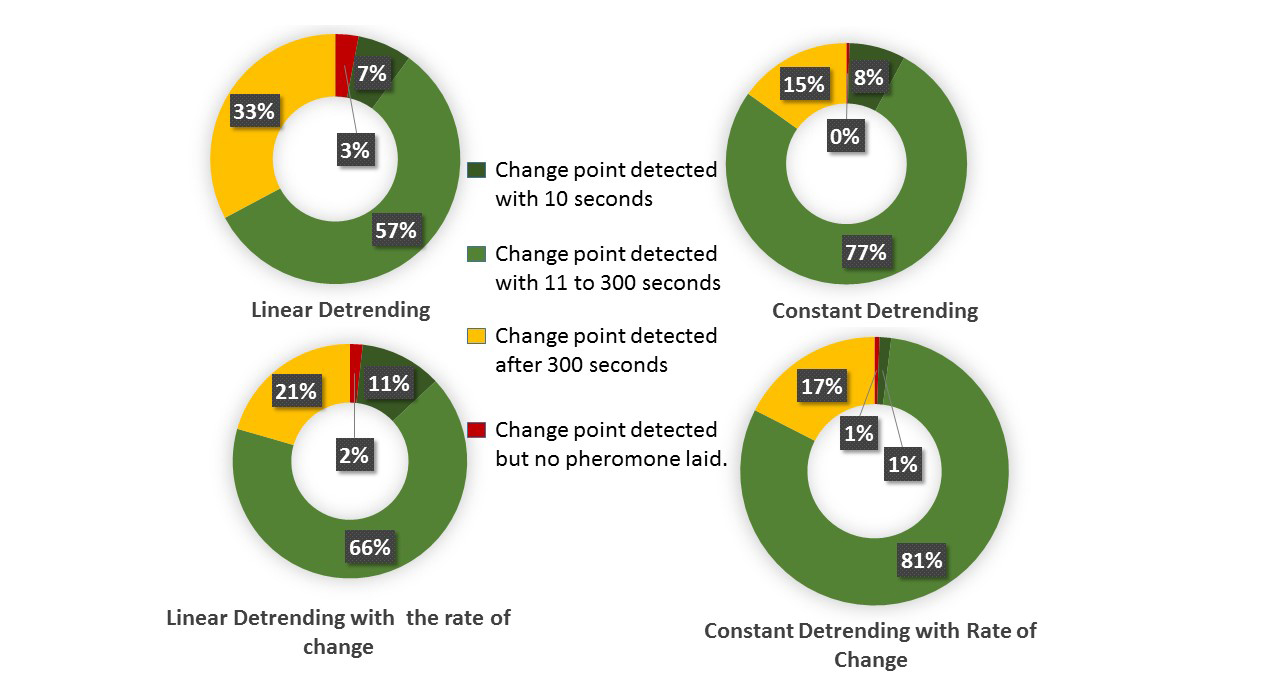
\includegraphics[width=\linewidth, height=0.4\textheight]{DonutCharts/Slide4.JPG}
	\caption{Efficiency chart for Change Point Detection Methods on sixteen small piles of 16 seeds. This result is generated from the simulated data of pheromone only environment, configured for \textit{P. Rugosus}}
\end{figure}
\begin{figure}[h]
	\includegraphics[width=\textwidth,height=0.6\textheight]{AllParameters/AllPlot.png}
	\caption{Comparison of Change Point Detection Methods without outliers for \textit{pheromone plus sitefidelity} environment . The time in seconds represents the difference between a pheromone laying event followed by a detection of change point in the foraging rate.}
\end{figure}
\begin{figure}
	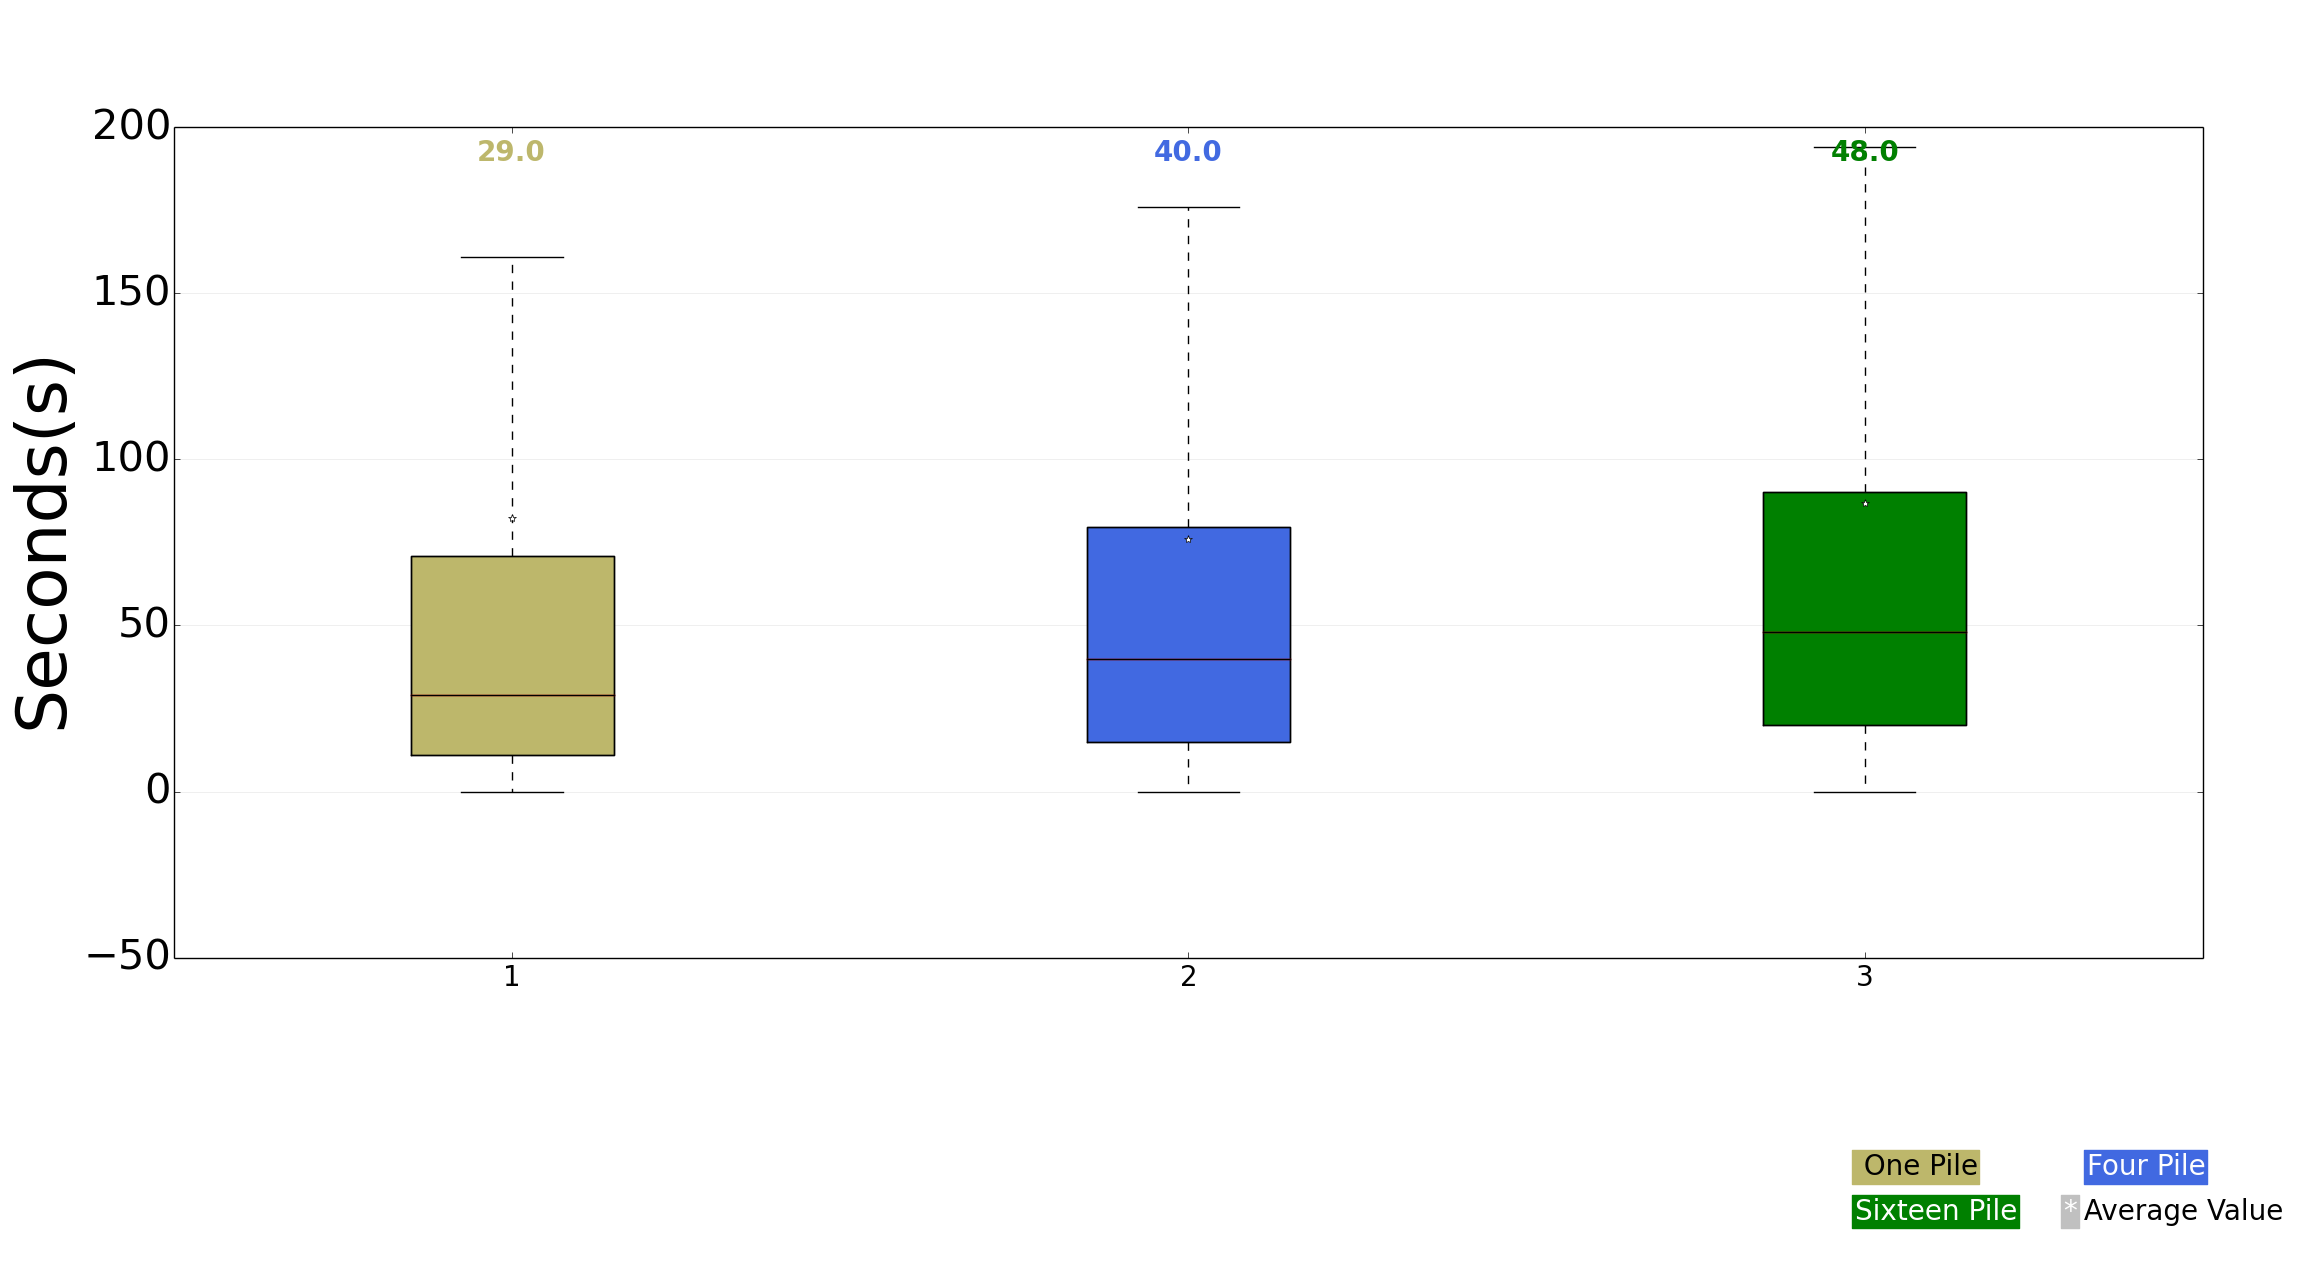
\includegraphics[width=\textwidth,height=0.4\textheight]{AllParameters/ConstantDetrendingNoOutlier.png}
	\caption{Enlarged view of efficiency of\textit{Method $\alpha$}. The time in seconds represents the difference between a pheromone laying event followed by a detection of change point in the foraging rate.}
\end{figure}
Figure $4.6$ shows the comparison of four different methods on a simulated environment with all parameters for \textit{P. Rugosus}. From this figure it is clearly visible that \textit{Method $\alpha$} does better in detecting the change points than any other methods. As a matter of fact, Method $\alpha$ does better in memory plus communication environment than the communication only environment.\par 
\begin{figure}[h]
	\begin{subfigure}{0.5\textwidth}
		\centering
		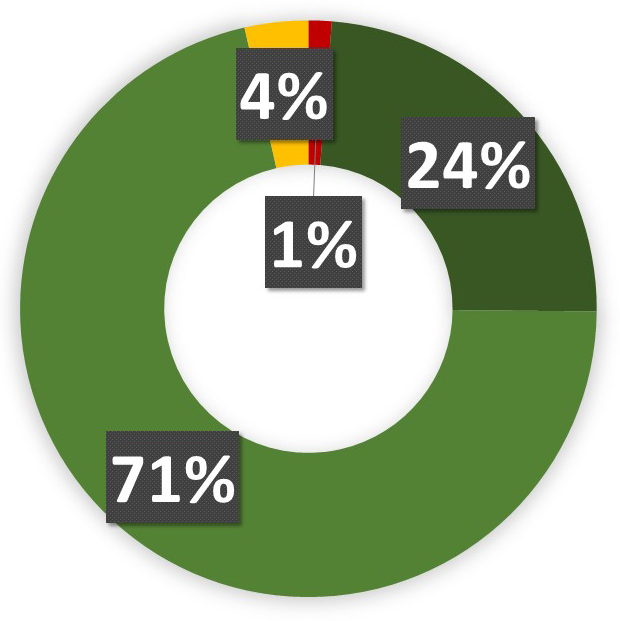
\includegraphics[width=0.5\linewidth]{DonutCharts/Slide11.JPG}
		\caption{}
		\label{fig:AllParam-Onepile}
	\end{subfigure}%
	\begin{subfigure}{0.5\textwidth}
		\centering
		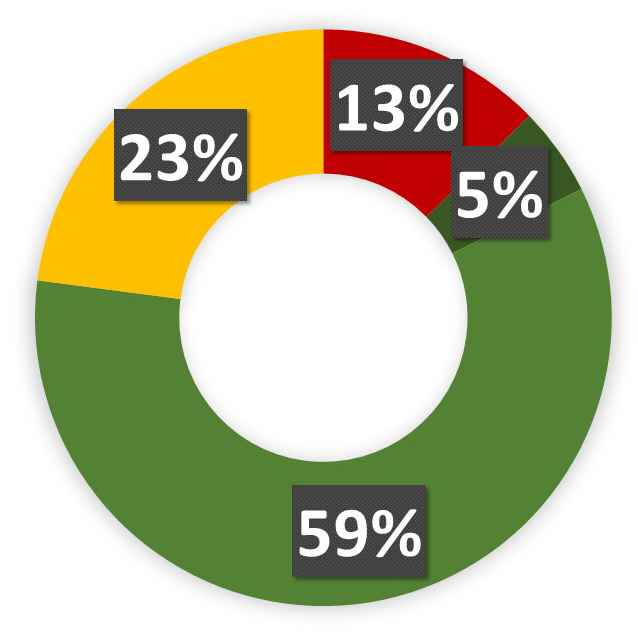
\includegraphics[width=0.5\linewidth]{DonutCharts/Slide12.JPG}
		\caption{}
		\label{fig:siteFidelity-OnePile}
	\end{subfigure}
	\caption{4.8(a) is the efficiency chart of the \textit{constant detrending} method for one large pile of 256 seeds. The data is generated from the simulation of pheromone plus site fidelity environment of \textit{P. Rugosus}. 
		4.8(b) is the efficiency chart for the constant detrending method for one large pile of 256 seeds. The figure is generated by analyzing the simulated data of sitefidelity only environment for \textit{P. Rugosus}. }
	\label{fig:fig}
\end{figure}
We have analyzed the efficiencies of all four methods for communication plus memory environmental settings. We observe that \textit{method $\alpha$} and \textit{method $\beta$} does significantly better than the other two methods. But in \textit{category C} and \textit{D} \textit{method $\alpha$} does better than \textit{method $\beta$}. We observe that the error is 0\% for \textit{method $\alpha$}, whereas it is 1\% for \textit{method $\beta$}. \textit{Method $\alpha$} also surpluses \textit{method $\beta$} in the combined result of category A and B. We observe, the similar pattern of performances for four piles and sixteen piles. \par 
Figure \textit{4.8(a)} is the efficiency chart for \textit{method $\alpha$} for one large pile on pheromone plus site fidelity environment. We skipped the results of other piles for \textit{P. Rugosus} as those have similar patterns of result. In figure \textit{4.8(b)} we demonstrate our model\textquotesingle s efficiency in detecting the change points when only site fidelity is used for \textit{P. Rugosus} on one large pile of 256 seeds.\par 
In memory only environment when no pheromone is used, agents use memory extensively. For this reason, when they start collecting seeds, their foraging rate goes up because of the extensive use of internal memory. Which is why \textit{constant detrending} method detects change points in site fidelity only environment also. So we have also measured the efficiency of all methods by measuring the difference between a use of site fidelity and followed by a change point. From figure 4.8(b), we have observed that 59\% of the time a change point is detected after the first use of site-fidelity.\par  
The performance rating is similar for \textit{P. Maricopa} and \textit{P. Desertorum}. Results for these two species are provided in the appendices.
\section{\label{section:Results from Field Data}Results from Field Data} 
We applied binary segmented cumulative sum change point detection method with constant detrending on the field data. The parameters are kept same as simulations for the change point detection method. We are able to detect change points in 6 experiments out of 11 for \textit{P. Desertorum}. For \textit{P. Maricopa}, we detected change points in 7 experiments out of 11 and for \textit{P. Rugosus} we are able to detect change points in 12 experiments out of 13. Table $4.2$ shows the detail of the results for field data.\par
\begin{table}[h]
	\footnotesize
	\begin{tabular}{|c|c|c|c|}
		\hline
		\multicolumn{4}{|c|}{\textit{P. Desertorum}} \\ \hline
		Experiment & One & Four & Sixteen \\ \hline
		DP15\_070709 & 6 & 4 & 2 \\ \hline
		DP10\_0606 & 6 & 4 & 2 \\ \hline
		DP14\_0606 & 6 & 4 & 1 \\ \hline
		DP15\_0604 & 6 & 0 & 2  \\ \hline   
		DP15\_0617 & 6 & 4 & 1 \\ \hline
		DPC\_070109 & 6 & 4 & 2  \\ \hline
	\end{tabular}
	\hfill
	\begin{tabular}{|c|c|c|c|}
	\hline
		\multicolumn{4}{|c|}{\textit{P. Maricopa}} \\ \hline
		Experiment & One & Four & Sixteen \\ \hline
		MP8\_0609 & 2 & 5 & 4 \\ \hline
		MP9\_0528 & 2 & 0 & 0 \\ \hline
		MP9\_0602 & 2 & 5 & 4 \\ \hline
		MP9\_0611 & 2 & 4 & 1  \\ \hline   
		MP9\_0620 & 2 & 5 & 4 \\ \hline
		MPE\_24Jul09 & 2 & 5 & 4  \\ \hline
		MPX\_0624 & 2 & 5 & 4  \\ \hline  
	\end{tabular}
	\hfill
	\\ \\
	\begin{center}
		\begin{tabular}{|c|c|c|c|}
			\hline
			\multicolumn{4}{|c|}{\textit{P. Rugosus}} \\ \hline
			Experiment & One & Four & Sixteen \\ \hline
			RP6\_0609 & 4 & 4 & 4 \\ \hline
			RP7\_0610 & 4 & 4 & 4 \\ \hline
			RP10\_0527 & 4 & 4 & 3 \\ \hline
			RP10\_0528 & 4 & 4 & 4  \\ \hline   
			RP10\_0604 & 3 & 0 & 3 \\ \hline
			RP12\_0602 & 4 & 4 & 4  \\ \hline
			RP14\_0610 & 4 & 4 & 0  \\ \hline  
			RP14\_0610 & 4 & 4 & 0  \\ \hline
			RP16\_0612 & 4 & 4 & 4  \\ \hline
			RP19\_0618 & 4 & 4 & 4  \\ \hline
			RS23\_0821 & 4 & 4 & 4  \\ \hline 
			RP17\_0617 & 4 & 4 & 4  \\ \hline 
		\end{tabular}
	\end{center}
	\caption{This table represents the number of change points detected in each of the field experiment of \textit{P. Desertorum}, \textit{P. Maricopa} and \textit{P. Rugosus}. For \textit{P. Desertorum}, we are able to detect change points in 6 experiments out of 11. For \textit{P. Maricopa} it is 7 out of 11. For \textit{P. Rugosus} it is 12 out of 13. The numbers conclude how many times change points are detected for a pile type in each experiment.}
\end{table}
From table $4.2$ we can see that \textit{P. Desertorum} is using much more pheromone for the large pile. It is discovering the pile more frequently than any other species. But the reason of having more change points in the foraging data of \textit{Desertorum} is, it discovers and looses pile very frequently. \textit{Maricopa} also detects the large pile. from the data is clearly visible that it does not looses the pile often. \par
 
We ran 500 simulated experiment to generate the data for each species. And we are able to detect change points in all of the experiments. This is because agents are programmed to forage despite the situations that harvester ants face. Foraging of harvester ants depends on many factors, including the weather, availability of resources and so many. As a result in some of the experiments we were not been able to detect enough amount of foraging from the ants. 